\documentclass[a4paper, 12pt]{article}

\usepackage{hyperref}
\usepackage{fullpage}
\usepackage[top=0.5in, bottom=1.5in, left=0.5in, right=0.5in, footskip=4em]{geometry}
\usepackage{amsmath}
\usepackage{fancyhdr}
\usepackage[usenames,dvipsnames]{xcolor}
\usepackage{pgfornament}

\usepackage[shortlabels]{enumitem}
\usepackage{xspace}
\usepackage{lastpage}
\usepackage{multicol}
\usepackage{blindtext}
\usepackage{titling}
\usepackage{standalone}
\usepackage{amsfonts}
\usepackage[framemethod=TikZ]{mdframed}
\usetikzlibrary{calc}
\usepackage{lineno}
\usepackage{amsthm}
\usepackage{amssymb}
\usepackage{mathtools}
\usepackage{datetime}
\usepackage[most]{tcolorbox}
\usetikzlibrary{tikzmark}
\linenumbers


%BEGIN_FOLD Commands
\newcommand{\half}{\frac{1}{2}}
\newcommand{\epv}[1]{\ensuremath{\left< #1 \right>}\xspace}
\newcommand{\variance}{\ensuremath{\text{Var}}}
\newcommand{\eout}{\ensuremath{E_\text{out}}\xspace}
\newcommand{\ein}{\ensuremath{E_\text{in}}\xspace}
\newcommand{\cx}{\ensuremath{\mathcal{X}}\xspace}
\newcommand{\cz}{\ensuremath{\mathcal{Z}}\xspace}
\newcommand{\real}{\mathbb{R}}
\DeclareSymbolFont{extraup}{U}{zavm}{m}{n}
\DeclareMathSymbol{\varheart}{\mathalpha}{extraup}{86}
\DeclareMathSymbol{\vardiamond}{\mathalpha}{extraup}{87}
\renewcommand{\heartsuit}{\textcolor{red}{\varheart}}
\renewcommand{\diamondsuit}{\textcolor{red}{\vardiamond}}
\newcommand{\definition}{\noindent\textbf{Def:} }
\newcommand{\theorem}{\noindent\textbf{Theorem:} }
\renewcommand{\proof}{\noindent\textbf{Proof:} }
\newcommand{\lemma}[1]{\noindent\textbf{Lemma #1:} }
\newcommand{\hint}{\textbf{Hint:} }
\newcommand{\basecase}{\noindent\textbf{Base Case:} }
\newcommand{\qedd}{\qed\newline}
\newcommand{\kwd}[1]{\textcolor{blue}{\textbf{\underline{#1}}}}
\newcommand\ColorBox[2][]{%
	\stepcounter{mybox}%
	\node[draw=red!70!black,fill=red!20,align=left,#1] (box\themybox) {#2};
}
\newcommand{\expl}[2]{%
	\underset{\substack{\uparrow\\\mathrlap{\text{\hspace{-1em}#2}}}}{#1}}
\newcommand{\st}{\text{ such that }}
%\newcommand{\qed}{\ensuremath{\blacksquare}}
%END_FOLD


%BEGIN_FOLD miscellaneious default
\makeatletter
% Make a copy of macros responsible for entering display math mode
\let\start@align@nopar\start@align
\let\start@gather@nopar\start@gather
\let\start@multline@nopar\start@multline
% Add the "empty line" command to the macros
\long\def\start@align{\par\start@align@nopar}
\long\def\start@gather{\par\start@gather@nopar}
\long\def\start@multline{\par\start@multline@nopar}
\makeatother
\setlength{\columnsep}{1cm}
%opening
\setlength{\abovedisplayskip}{-\baselineskip}%
\setlength{\abovedisplayshortskip}{\abovedisplayskip}%

\pagestyle{fancy}
\renewcommand{\headrulewidth}{0pt}
\lfoot{\small{\course}: Week \weekno}
\rfoot{\small{\thetitle}}
\rhead{}
\cfoot{\pgfornament[height=1em, ydelta=-0.4em]{11} \thepage of \pageref{LastPage}  \pgfornament[height=1em, ydelta=-0.4em]{14}}

\DeclareMathOperator{\sign}{sign}
\newcommand{\vect}[1]{\ensuremath{\mathbf{#1}}\xspace}

\tikzstyle{every picture}+=[remember picture]
\newcommand{\bwgrid}[1]{
	\def \aaa #1
	
	\foreach \y in {0,1,2} {
		\foreach \x in {0,1,2} {
			\pgfmathsetmacro{\clr}{\aaa[\x][\y]}
			%\message{aaa \clr}
			\definecolor{MyColor}{rgb}{\clr,\clr,\clr}
			\path[fill=MyColor] (\x,\y) rectangle ++(1,1); 
		}
	}
	\draw[step=1cm,very thin] (0,0) grid (3,3);	
}

\setenumerate{label=\alph*.)}
\definecolor{db}{RGB}{100,65,23}
\newtheoremstyle{examplestyle}% name
{}%         Space above, empty = `usual value'
{}%         Space below
{}% Body font
{}%         Indent amount (empty = no indent, \parindent = para indent)
{}% Thm head font
{}%        Punctuation after thm head
{\newline}% Space after thm head: \newline = linebreak
{\textbf{\textcolor{db}{\thmname{#1}\thmnumber{ #2}:} \thmnote{ #3}}}%         Thm head spec
\theoremstyle{examplestyle}

\newtheorem{examplethm}{Example}
\newenvironment{example}[1][]{\begin{mdframed}[style=example]\begin{examplethm}[#1]}{\end{examplethm}\end{mdframed}}

\newenvironment{example*}[1][]{\begin{mdframed}[style=example]\begin{examplethm}[#1]\end{examplethm}}{\end{mdframed}}
\newenvironment{Figure}
{\par\medskip\noindent\minipage{\linewidth}}
{\endminipage\par\medskip}
\newenvironment{formula}{
	\begin{mdframed}[style=formula]
	}{
\end{mdframed}}
%END_FOLD

\newcommand{\course}{Discrete Math}
\title{Proof Techniques}
\newcommand{\weekno}{1}

\begin{document}
\begin{center}
	\textcolor{orange}{\textsc{\course}}\\
	\huge\textbf{\textsc{\thetitle}}\\
	\small\textcolor{gray}{Last updated:\, \today \, \currenttime}\\
	\pgfornament[width=0.7\textwidth, color=white!30!black]{89}
\end{center}

\begin{multicols}{2}
\section*{Axiomatic Proof}
The notion of proof dated back to Euclid and Archimedes\footnote{The story of his death is quite intriguing. The city got invaded soldier comes in to his house. He refused to surrender since he is working on math.}. The word axiom means something that we assume to be true. You could however argue whether the axiom applied to the problem we are trying to solve or not. If it does then that is good, but if it does not you pick the wrong set of axiom.

The axiom usually contains trivial stuff like you can commute addition ($a+b = b+a$) or if $a =b$ and $c=d$ then $a+c = b+d$ etc. Another example would be that the area is the same for every observer no matter who observe it or no matter how we move or rotate it.\footnote{This is only true in flat space.}.

The idea of proof is to show that the statement is true/false beyond reasonable doubt. Let us work on our first proof

\noindent\theorem Given a right triangle
	\begin{center}
		\begin{tikzpicture}
		
		\draw (0,0)--(0,2) node[midway,left]{$a$};
		\draw (0,0)--(4,0) node[midway,below]{$b$};
		\draw (0,2)--(4,0) node[midway,above]{$c$};
		
		\end{tikzpicture}
	\end{center}
	Then, the length of all three sides are related by
	\[
		c^2 = a^2 + b^2
	\]
	\proof First, we pieces the tringle in a useful way\footnote{This proof is credited to President Garfield.}
	\begin{center}
		\begin{tikzpicture}
		
		\draw (0,0)--(0,2) node[midway,left]{$a$};
		\draw (0,0)--(4,0) node[midway,below]{$b$};
		\draw (0,2)--(4,0) node[midway,above]{$c$};
		
		\draw[red] (4,0)--(6,0) node[midway,below]{$a$};
		\draw[red] (6,0)--(6,4) node[midway,right]{$b$};
		\draw[red] (4,0)--(6,4) node[midway,above]{$c$};
		
		\draw[dashed, blue] (0,2) -- (6,4);
		\end{tikzpicture}
	\end{center}
	
	We can calculate the area of this trapezoid in two ways
	\[
		A_1 = \half(b+a)\times(b+a)
	\]
	or we can add up the area of all triangles
	\[
		A_2 = \half a b + \half a b + \half c^2
	\]
	Since they are the same area,
	\begin{align}
		A_1 &= A_2 \\
		\half\left(b^2 + a^2 +2ab\right) &= \half ab + \half ab + \half c^2\\
		a^2 + b^2 &= c^2
	\end{align}
	\qedd
	
You can see from the above proof that the idea of the proof is that we start from knowledge which we know to be true: how to find the area. Then we build the idea in a small step making sure each step is reasonably obvious to the reader. Then after enough steps we should reach the final goal. Think of this as trying to explain to your friends in this class. Make sure that if your friends read this proof then he/she should be convinced what you are trying to say.

For a given proposition there are usually many ways to write it. Writing a good proof is a work of art. In this chapter, you will see a couple of common proof techniques. 

Let us do a couple more examples.

\noindent\definition An integer $a$ is \kwd{even} iff $$\exists n \in I \st 2n = a$$

\noindent\definition An integer $a$ is \kwd{odd} iff $$\exists n \in I \st 2n+1 = a$$

For example, $6$ is even since if $n=3$ then we get $2\times 3 = 6$. $7$ is odd since $n=3$ then we get $2\times3 + 1 = 7$.

Let us use these definitions to show that

\noindent\theorem Assume that $x$ is even and $y$ is odd then $xy$ is even.

\noindent\proof
Since $x$ is even this means, by definition above, that
\[
	\exists n \in I \st 2n = x
\]
Let us call the number $n_x \in I$
\[
	2n_x = x
\]

Similarly, for $y$ since it is odd, by definition, we can find an integer $n_y$ such that
\[
	2n_y + 1 = y
\]

Consider the product of the two
\begin{align*}
 xy & = 2n_x \times (2 n_y + 1)\\
 & = 2 (n_x \times (2 n_y + 1) )\\
 & = 2 m
\end{align*}
Since $m$ is a product of integers, $m$ is an integer. Thus,$$\exists m \in I \st 2m = xy.$$

Therefore, $xy$ is even.\qedd

It is very useful if you know exactly where exactly you are going. Otherwise you will get lost. The above prove illustrates this point. If you read the theorem for the first time, you will definitely have the question in your mind ``What exactly do I need to do". As you can see, we need to show that given all these assumptions, the \kwd{result must be even}. So, we really need to show that the product is even. Then you will ask youself: what exactly do I need to show to show that something is even. To do that you will need to refer to the \kwd{definiton}. The definition says an integer even iff there is an integer $n$ such that $2n=$that number. So, our goal is to show that the product is really 2 times some integer.

Let us do the next example:

\noindent\theorem If $x$ is odd and $y$ is odd then $xy$ is odd.

\noindent\proof
Before we go on, remember that our goal is to show that $xy$ is odd that is
\[
	xy = 2m +1
\]
for some integer $m$.

Since $x$ and $y$ are odd then there exists integer $n_x$ and $n_y$ such that
\begin{align*}
	x &= 2n_x +1 \\
	y &= 2n_y +1
\end{align*}

Let us consider the product
\begin{align*}
	xy &= (2n_x+1)(2n_y+1)\\
	   &= 4n_xn_y +2n_x + 2n_y +1\\
	   &= 2(2n_xn_y +n_x + n_y) +1
\end{align*}

Since ther term in the parenthesis is just a sum of integers, it is an integer. Therefore
\[
xy = 2m+1
\]
where $m\in I$ and $m = (2n_xn_y +n_x + n_y)$. Thus, $xy$ is odd. \qedd

As an exercise, to write proof to show that odd+odd = even, even+odd = odd etc.

\section*{Proof By Cases}

This is the bruteforce method for proof. It works quite well. We kind of did it before when we show the logical idneity that $$(P\to Q) \land (Q\to P) = P \iff Q$$. We showed that by building an exhuastive list of possible $P$ and $Q$ then we show that the left hand side and the right hand side are equal for all possibility of $P$ and $Q$.

Let us consider a less trivial example of proof by case. Let us define a couple things first.


\noindent\definition A \kwd{group} of $n$ strangers means a set of $n$ people where none of them are friend on facebook.


\noindent\definition A \kwd{club} of $n$ people means a set of $n$ people where
\[
	\forall a,b \in \text{club}, a\ne b; a \text{ and } b \text{ are friends on facebook}.
\]In other words, it just means that everyone in the club knows everyone else in the club.

Now here comes our theorem.

\theorem Every collection of 6 people includes either a club of 3 people \emph{or} a group of 3 strangers.

\begin{center}
	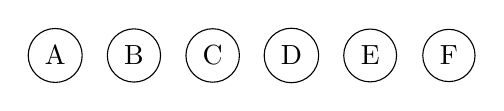
\begin{tikzpicture}
\node()[draw, circle] at (0,0) {A};
\node()[draw, circle] at (1,0) {B};
\node()[draw, circle] at (2,0) {C};
\node()[draw, circle] at (3,0) {D};
\node()[draw, circle] at (4,0) {E};
\node()[draw, circle] at (5,0) {F};
\end{tikzpicture}
\end{center}

\noindent\proof
The goal here is to show that you can form a club or a group of strangers for all the possibilities of friendship among these six people. You will learn later in the course that there are $2^{15}$ cases(assuming people are distinct).\footnote{There are actually 156 if you discount all the homomorphism. \url{https://oeis.org/A000088}} But that is a lot. So we need to be a little bit smart in doing cases analysis.


Let us consider $A$. So we have two cases:
\begin{enumerate}[1)]
	\item At least 3 people are friend with A. [A has 3-5 friends]
	\item At least 3 people are NOT friend with A. [A has 0-2 friends]
\end{enumerate}



Let us consider case 1). If we consider the three people, who are friend with A there are two cases.
\begin{enumerate}[leftmargin=1in]
	\item[Case 1.1:] \emph{None} of the people who knows A know each other. Then these three people form a group of Stranger. The theorem is satisfied.
	\item[Case 1.2:] \emph{Some} pair of people who knows A know each other. Then the pair of people and A form a club of 3 people.
\end{enumerate}

Now consider case 2). If we consider the 3 people who doesn't know know A, there are 2 cases: 
\begin{enumerate} [leftmargin=1in]
	\item[Case 2.1] \emph{All} 3 people know each other. Then these 3 people form a club.
	\item[Case 2.2] \emph{At least one pair} of these 3 people don't know each other. Then this pair of people and A form a group of 3 strangers.
\end{enumerate}

Since we have covered every case, we are done with the proof.\qedd

\section*{Proof By Contradiction}
Suppose we want to show that blackhole doesn't exist on the earth surface, we can use the following argument: if blackhole exists on earth then the earth would be gone. But the earth is still here therefore blackhole doesn't exists.

This kind of argument is called proof by contradiction. It goes along the the line of assuming that the proposition is not true then it will lead to some contradiction/break something that we know to be true.

\noindent\theorem An integer cannot be both odd and even.

\noindent\proof Proof by contradiciton is perfect for this kind of things. We do not have much handles to prove that something doesn't exists. Proof by contradiction gives us a handle.

So, first we will assume for the sake of contradiction that the proposition is false. That means
\[
	\exists x \in I\;\;\text{where } x \text{ is both odd and even}
\]

Then, we hope that $x$ we assume to exists will lead to some contradiction.

Since $x$ is even. This means
\[
	x = 2 n_E
\]
for some integer $n_E$.

And since $x$ is also even. This means
\[
	x = 2 n_O + 1
\]
for some integer $n_O$.

However, since
\[
	x = 2n_E = 2n_O + 1,
\]
we have
\[
	n_E = n_O+\half.
\]

This is a contradiction since this means that $n_E$ and $n_O$ cannot be both integer since one is a half more than the other.

Therefore, an integer cannot be both odd and even.\qedd

Let us consider a more challenging one

\noindent\theorem If $a,b,c \in \mathbb{O}$ where $\mathbb{O}$ means set of all odd number then\[
	ax^2 + bx + c = 0
\]
has no integer solution.

\noindent\proof We will prove this by contradiction. Let assume for the sake of contradiction that there exists an integer solution $x$. Then, $x$ must be odd

If $x$ is even then \begin{center}
	$ax^2 +bx +c$ = even + even + odd = odd
\end{center}. But, 0 is not an odd number. Therefore, even $x$ cannot be a solution.

If $x$ is odd then \begin{center}
	$ax^2 +bx + c$ = odd + odd + odd = odd
\end{center}. But, 0 is not an odd number. Therefore, odd $x$ cannot be a solution.

Thus, $ax^2 + bx + c = 0$ has no integer solution.\qedd

Let us consider a classic one.

\noindent\definition A number $x$ is \kwd{rational} if $\exists p,q \in I$ such that
\[
	x = \frac{p}{q}
\]
\noindent\definition A number $x$ is \kwd{irrational} if $\forall p,q \in I$
\[
	x \ne \frac{p}{q}
\]

\noindent\theorem $\sqrt{2}$ is irrational.

\noindent\proof Let us assume for the sake of contradiction that $\sqrt{2}$ is \emph{rational}.

This means that $\exists p,q \in I$ such that
\[
	\sqrt{2} = \frac{p}{q}
\]

Furthermore, we require that $p$ and $q$ \emph{has no common factor}. If it does then, we will cancel them in the division.

Squaring both sides we have
\begin{equation}
	p^2 = 2q^2
	\label{eq_sq21}
\end{equation}

This imply that $p$ must be even by definition of even. Thus
\[
	p = 2m
\]

Plugging this back in to Equation \ref{eq_sq21} we got
\begin{align*}
	4m^2 &= 2 q^2\\
	2m^2 &= q.
\end{align*}

The last line tells us that $q$ must also be even.

However, from above, we know that $p$ and $q$ has no common factor. Thus, $p$ and $q$ cannot be both even. This leads to a contraction.

Therefore, $\sqrt{2}$ is irrational.\footnote{This proof has a very interesting history. \url{https://en.wikipedia.org/wiki/Hippasus}}
\qedd

Let us consider another classic one credited to Euclid from 300BC but it still stands today as an example of clever reasoning.

\noindent\theorem There are infintely many prime numbers

\noindent\proof Let us assume for the sake of contradiction that there are finite number of prime number. Let us call the set of \emph{all} prime nubmer $\mathbb{P}$.

Since there are finite number of prime we can write $\mathbb{P}$ as
\[
	\mathbb{P} = \{p_1, p_2, p_3, \ldots, p_n\}
\]
where $p_n$ is the \emph{biggest} prime number.

However, let us consider the number
\[
	q = p_1p_2p_3\ldots p_n + 1 
\]

This number is bigger than $p_n$ so it cannot be a prime. Thus, $\exists p_k$ that divides $q$. Thus $\exists c \in I$

\[
q = cp_k = p_1p_2p_3\ldots p_{k-1} p_k p_{k+1} \ldots p_n + 1 
\]

Dividing both sides by $p_k$ we have
\[
c = p_1p_2p_3\ldots p_{k-1} p_{k+1} \ldots p_n + \frac{1}{p_k}
\]

This is not possible since the left hand side is integer but the right hand side is not an integer.

Thus, we have a contradiction since $q$ must be either prime or non prime.

Therefore, there are infinitely many prime numbers.\qedd

\section*{Contrapositive Proof}
Supposed you are trying to show that:
\begin{center}
	Dry Grass $\implies$ Not Raining.
\end{center}
That is everytime your lawn is dry that means it didn't rain.

Supposed you can show the contrapositive that
\begin{center}
	Raining $\implies$ Wet Grass
\end{center}
That is everytime it rains you lawn will be wet. Then your job is done.

Why is this true? If you think about it if we know for a fact that everytime it rains your grass is wet. Then, you know for a fact that on a raining day, dry grass is not possible since it would violate what we know about Rains $\implies$ Wet. Therefore, the only possibility left for having dry grass is that it didn't rain.

In a formal logic sense, this is the same thing as using
\[
	P \to Q = \sim Q \to \sim P.
\]

We worked out earlier that the two statements are equivalent. Thus, if we can show that the right hand side is true then the left hand side is automatically true. 

In our grass and rain example, $P$ is Dry Grass and $Q$ is Not Raining and we are trying to show that
\begin{center}
	Dry Grass($P$) $\implies$ Not Raining($Q$)
\end{center}
by using the proving the fact that
\begin{center}
	Raining($\sim Q$) $\implies$ Wet Grass($\sim P$)
\end{center}

This sometimes make the proof much easier to contruct. Let us look at an example:

\theorem $\forall x \in I$, If $7x+9$ is even then $x$ is odd.

\proof Let us do this first by doing a direct proof.

Since $7x+9$ is even that means $\exists n \in I$
\begin{align*}
	7x+9 &= 2n\\
	7x &= 2n-9\\
	x &= 2n - 6x -9\\
	x & = 2(n-4x -5) +1
\end{align*}

Therefore $n$ is odd. \qedd

\proof We will now do this by contrapositive. So we want to prove the contrapositie of the propostiion which is
\begin{center}
	If $x$ is even, then $7x+9$ is odd. 
\end{center}

$x$ is even. Thus, $7x$ is even. Therefore $7x+9$ is odd.\qedd

You can see that for this proposition contrapositive make our lives much easier.

\theorem If $x^2-6x+5$ is even then $x$ is odd.
\proof I am not even sure how to do direct proof for this one. But the contrapositive is easy to prove. The contrapositive of this proposition that we want to prove is
\begin{center}
	$x$ is even then $x^2-6x+5$ is odd.
\end{center}
This is easy since
\[
	\expl{x^2}{\text{even}} - \expl{6x}{\text{even}} + \expl{5}{\text{odd}} = \text{odd}
\]
\qedd

Let us look at another example how this is helpful.

\definition Let $n,x \in I$, $n | x$ reads $n$ divides $x$. This means that $\exists c\in I$ such that $x = cn$.

\definition $n \nmid x$ reads $n$ does not divide $x$. This means that $\forall c \in I$, $x \ne cn$. Or in plain text it means $x$ does not contain $n$ as a factor.

\theorem Let $a,b,n \in I$.  If $ n \nmid ab$ then $n\nmid a$ and $n \nmid b$

\proof Let us prove the contrapositive of the proposition which is
\begin{center}
	If $n | a$ or $n | b$ then $n | ab$.
\end{center}

Notice how and is changed to or. If you think about the negation of logic this is what you want.

So, first, if $n|a$ then
\[ a = cn. \]
Therefore, multiplying $b$ on both sides gives
\[
	ab = cnb = n(cb).
\]
Therefore, $n | ab$.

The proof for the case $n|b$ is similar to the case where $n|a$. This is left for the reader as an exercise.

Therefore, the contrapositive is true. Thus,
\begin{center}
If $ n \nmid ab$ then $n\nmid a$ and $n \nmid b$
\end{center}
\qed
\section*{Iff}

This section is a little sidenote for how to show if-and-only-if. This is best illustrated by an example.

\theorem Let $a,b \in I$, then $ab$ is even if and only if $a$ is even or $b$ is even.

\proof To prove that $P$ iff $Q$ we need to show that $P$ implies $Q$ and $Q$ implies $P$. Specifically, we need tho show two things:
\begin{enumerate}
	\item $P \to Q$. $ab$ is even $\to$ $a$ is even or $b$ is even.
	\item $Q \to P$. $a$ is even or $b$ is even $\to$ $ab$ is even.
\end{enumerate}

To make this prove we are going to use lemma. You can think about lemma as mini theorem or helper function.

\lemma{1} $ab$ is even $\to$ $a$ is even or $b$ is even.
\proof
The first direction we can use contrapositive of the proposition above which is
\begin{center}
	$a$ is odd and $b$ is odd $\to$ $ab$ is odd.
\end{center}
We have proved this before \qedd.


\lemma{2} $a$ is even or $b$ is even then $ab$ is even.
\proof 

If $a$ is even then $a=2n$ and $ab=2(nb)$. Therfore, $ab$ is even.

If $b$ is even then $b=2n$ and $ab=2(nb)$. Therfore, $ab$ is even.
\qedd


Back to our main theorem. By Lemma 1 and Lemma 2,
\begin{center}
	$ab$ is even if and only if $a$ is even or $b$ is even.
\end{center}


\qedd

\section*{Pigeon Hole Principle}

This is a simple statement saying that

\theorem If there are more pigeons than the hole, then at least one hole has more than one pigeon.

\proof Left for the reader as an exercise. Use contrapositive.
\qedd

Eventhough, it seems like a trivial statement. It crops up everytime in the place you never expect. For example,

\theorem At least two people in Bangkok have the same number of hair.

\proof For the area of our sculp it can accomodate at most 300,000 hair but there are 10 million people in bangkok. If we think about the hair as holes and people as pigeons. Then, pigeon hold principle guarantees that there is at least one hair hole that has more than one people in it.\qedd

\theorem A group of $N$ people will have at least two people who have the same amount of friend(mutual) within the group.

\proof We can't exacly apply pigeon hole principle here since the number of friends in the group is from $0$ to $N-1$ which is $N$ slot yet we have $N$ people.

But, if we consider two cases:
\begin{enumerate}
\item If at least one person have zero friend, then no one can have $N-1$ friend. Then the number of friends possibility goes from $0$ to $N-2$ which means there are $N-1$ slots and there are $N$ people. The pigeon hole principle tells us that at least two people have the same amount of friend.
\item If no one has zero friend, then the possibility of number of friend then go from $1$ to $N-1$ which means there are $N-1$ possibilities. Since we have $N$ people, the pigeon hole principle tells us that at least two people have the same amount of friends.
\end{enumerate}
\qedd


\section*{Bonus Card Tricks}

\textbf{Spoiler Alert!!}.
To get the full experience don't read this before the class. Get fooled first and use this as reference.

\subsection*{Klondike Shuffle}

It's a self-working magic trick. So here is the effect:
\begin{enumerate}
	\item Have a volunteer(victim) pick any card. Take a peek and place it back face down on the top of the pile.
	\item Now you will need to place the top 26 cards down on the table one by one(important). This means the picked card will be at the very bottom. The left over 26 cards form another pile.
	\item At this stage we have two piles of 26 each. Where one of them has the selected card at the bottom. We will call this pile $A$ and the other pile $B$.
	\item Have the volunteer pick his/her favorite number, $p$ between 1 to 26. Then remove that many cards from pile $B$.
	\item Put pile $A$ on top of pile $B$.
	\item Then, we do the Klondike Shuffle. Klondike is ice-cream sanwich. This is done by removing the top and the bottom card as a pair and put them into another pile. Do this for the whole deck. For example, if the card order is (top)1,2,3,4,5,6(bottom) after Klondike shuffle, we should end up with 3,4,2,5,1,6.
	\item Give the volunteer the klondike-shuffled deck. Ask the volunteer again what was his/her favorite number $p$. The chosen card will be at the $p$-th position from the top.
\end{enumerate}

For this kind of trick, to understand how it works, all we need to do is just to keep track of where the chosen card is. 

\theorem Given two pile of $n$ card each one with the chosen card at the bottom. The card trick works.

\proof 
\begin{itemize}
	\item Let the number the volunteer picked to be $p$. Since we remove $p$ card from the pile without the chosen card. We end up with two pile.
		\begin{itemize}
			\item Pile $A$: $n$-card pile with the chosen card at the bottom.
			\item Pile $B$: $n-p$-card pile.
		\end{itemize}
	\item Since we put pile $A$ on top of pile $B$. That means the deck consists of $n-1$ card on the top, then our chosen card, then $n-p$ cards. The total nubmer of cards is $2n-p$.
	\item After $n-p$ Klondike shuffle, the chosen card will be the at the bottom of the leftover deck in our hand. 
	\item Since the chosen card will be place down next, all we need to compute now is the total number of cards left in our hand.
	\item We did $n-p$ Klondike shuffle, which means we have placed $2(n-p)$.
	\item The total number of cards was $2n-p$ that means we have $(2n-p) - 2(n-p) = p$ cards left in our hand.
	\item Since we continue to klondike-shuffle the rest of the deck. This means that the chosen card will appear at the $p$ position from the top of the klondiked-shuffle deck.
\end{itemize}
\qedd

\subsection*{Trolling people}

As a follow up to this trick after we learn how it works. This will throw a lot of people off guard. The idea is instead of putting pile $A$ on top of pile $B$. We do the opposite: putting $B$ on top of $A$. This means that the chosen card would be at the very bottom of the klondike-shuffled deck and not at the the $p$ position from the top. Then we can pretend the oh wait the trick does work. Then, show the bottom card aka the chosen on as dramatic as you like.

\subsection*{Red Pile and Black Pile}

Here is a variant of the red pair, black pair trick we proof earlier. Here is the effect.
\begin{enumerate}
	\item Have the spectator shuffle the deck.
	\item Open one card at the top. 
		\begin{itemize}
			\item If it's red, place the red card face up on the left. Then place the next card face down next to the face up red card.
			\item If it's black, place the red card face up on the right. Then place the next card face down next to the face up black card.
		\end{itemize} 
	\item Continue with the earlier procedure for the rest of the deck. We should end up with 4 pile.
		\begin{itemize}
			\item Face up red card pile
			\item Face down cards that were after red cards. ($R$ pile)
			\item Face up black card pile
			\item Face down cards that were after black cards. ($B$ pile)
		\end{itemize}
	\item Give the $R$ pile to one spectator $S_r$ and the $B$ pile to another spectator $S_b$.
	\item Have $S_r$ pick a number $p_r$.
	\item Then told $S_r$ to give $p_r$ cards to $S_b$. 
	\item Then have $S_b$ give $p_r$ cards back to $S_r$. They both end up with the same number of cards each of them had at the beginning. They do not necessarily have the same number of cards.
	\item Have them exchange equal number of cards as many times as they like.
	\item Ask $S_r$ to count number of red cards and ask $S_b$ count the number of black cards.
	\item The two numbers will be the same.
\end{enumerate}

\proof The proof is left to the reader as exercise. This is a euphimism for the fact that I'm too lazy to write it down.


\end{multicols}




\end{document}
